
\section{Architektur}
\label{Architektur}

In diesem Kapitel wird die Architektur unserer Applikation und die Schnittstellen zu den Umsystemen besprochen.
Als Anhaltspunkt wird das C4 Modell \cite{c4model} von Simon Brown verwendet.
In einem ersten Schritt wird unsere Applikation "`ÖV-Güteklassen 2018"' in den Kontext des grösseren Systems gesetzt.
Anschliessend teilen wir das System "`ÖV-Güteklassen 2018"' in einzelne Container und den zentralen Container "`ÖV-Güteklassen 2018 Generator"' in einzelne Komponenten auf.

\subsection{Systemkontext}
\label{Architektur:Systemkontext}

In Abbildung \ref{fig:system-context-diagram} ist gestrichelt eingerahmt das System "`ÖV-Güteklassen 2018"' zusammen mit den dazugehörigen Umsystemen dargestellt.
Die Pfeile bedeuten, dass ein System in Richtung der Pfeilspitze Anfragen an ein anderes System sendet.
Die Daten fliessen dementsprechend in die entgegengesetzte Richtung.

\begin{figure}[ht]
    \centering
    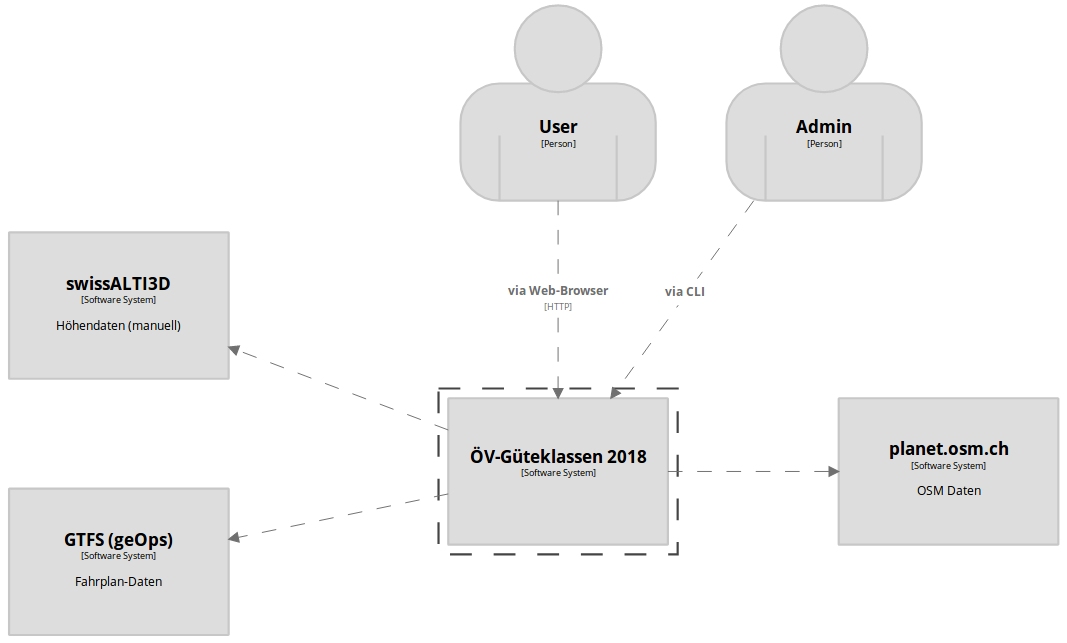
\includegraphics[width=1\linewidth]{projectdoc/img/systemcontext-diagram.png}
    \caption[Systemkontextdiagramm]{Systemkontextdiagramm ÖV-Güteklassen 2018}
    \label{fig:system-context-diagram}
\end{figure}

Im Folgenden werden die Umsysteme sowie die Beziehungen zu unserem System "`ÖV-Güteklassen 2018"' genauer beschrieben.

\subsubsection{swissALTI$^{3D}$}
\label{subsystem:swissALTI3D}

Als \gls{Terrainmodell} wird swissALTI$^{3D}$, ein Produkt von swisstopo~\cite{swissalti3d_swisstopo}, verwendet.
Dieses wird manuell vom Admin bezogen, da der Datensatz mit ca. 120GB für ein Download über das Web-\ac{API} zu gross ist und da die Daten keinem stetigem Wandel unterstellt sind.
Diese werden von swisstopo~\cite{swissalti3d_swisstopo} in einem Nachführungszyklus von 6 Jahren aktualisiert.

Das \gls{Terrainmodell} wird anschliessend in die Routing-Engine integriert, wo die Höhenunterschiede für die Kostenberechnung einer Route verwendet werden können.

\subsubsection{GTFS}
\label{subsystem:GTFS}

Die Fahrplandaten werden von der SBB regelmässig im HAFAS-Format publiziert.~\cite{sbb_hafas_spec}
Diese werden von geOps~\cite{geops_fahrplandaten} in das offene und einfacher handhabbare Format \ac{GTFS}~\cite{gtfs_spec} konvertiert und kostenfrei publiziert.~\cite{geops_fahrplandaten}
Diese können im CSV-Format für eine Speicherung in einer relationalen Datenbank bezogen werden.
Das Datenmodell ist in Abbildung \ref{fig:GTFS_data_model} ersichtlich.

\begin{figure}[ht]
    \centering
    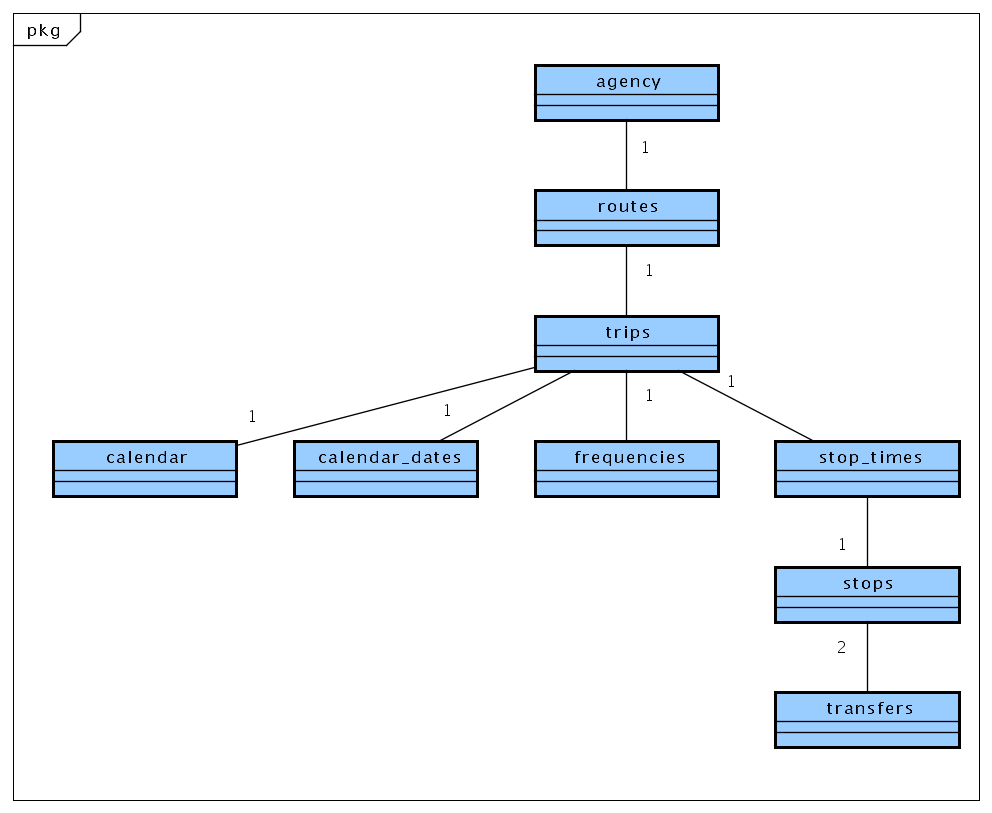
\includegraphics[width=1.0\linewidth]{projectdoc/img/GTFS_data_model}
    \caption[GTFS Datenmodell]{GTFS Datenmodell}
    \label{fig:GTFS_data_model}
\end{figure}

\subsubsection{planet.osm.ch}
\label{subsystem:planet.osm.ch}

Für die Berechnung der ÖV-Güteklassen benötigt es aktuelle Kartendaten, um die Erreichbarkeiten von Haltestellen entlang dem Strassennetz zu analysieren.
Dazu bieten sich Daten von \ac{OSM} ideal an, da sie frei verfügbar sind und kontinuierlich aktualisiert werden.

Unter planet.osm.ch~\cite{planet_osm_ch} werden täglich aktualisierte \ac{OSM}-Daten der ganzen Schweiz bereit gestellt.
Die Daten sind im \ac{PBF} und werden mit entsprechenden Tools in eine relationale Datenbank importiert, wo sie von einer Routing-Engine genutzt werden können.


\subsection{Container}
\label{Architektur:Container}

In der Abbildung \ref{fig:container-diagram} ist das System "`ÖV-Güteklassen 2018"', wie es in im \nameref{Architektur:Systemkontext} vorkam, in einzelne Container aufgespalten.
Im Folgenden werden die einzelnen Container genauer beschrieben.

\begin{figure}[ht]
    \centering
    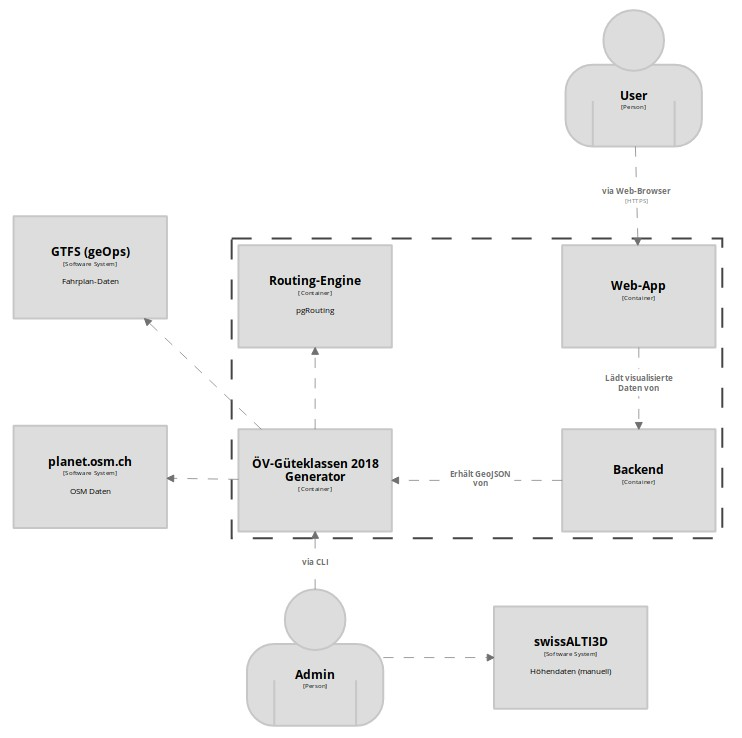
\includegraphics[width=1.0\linewidth]{projectdoc/img/container-diagram.png}
    \caption[Containerdiagramm]{Containerdiagramm ÖV-Güteklassen 2018}
    \label{fig:container-diagram}
\end{figure}
% TODO: Use Express export instead of a screenshot

\subsubsection{ÖV-Güteklassen 2018 Generator}
\label{container:generator}

Der "`\acs{ÖV}-Güteklassen 2018 Generator"' stellt das Kernstück der Berechnung der \acs{ÖV}-Güteklassen 2018 aufgrund der Spezifikation dar.
In der Abbildung \ref{fig:layer_diagram_generator} ist das Schichten-Diagramm ersichtlich.
Die Kernlogik der Berechnung befindet sich in der Schicht \nameref{layer:business}.
Der Generator agiert auf unterschiedlichen Datenquellen, so werden Fahrplandaten (\nameref{subsystem:GTFS}), ein Routing-Graphen (\nameref{subsystem:planet.osm.ch} und \nameref{container:Routing-Engine}) und ein Terrain-Modell (\nameref{subsystem:swissALTI3D}) verarbeitet und genutzt.
Die Komponente setzt voraus, dass vor dem Starten diese Daten im System vorhanden sind.
Die Integration dieser Daten ist in der Schicht \nameref{layer:integration} angesiedelt.
Die Interaktionen mit dem User sind in der Schicht \nameref{layer:ui} und die Resultate werden in der Schicht \nameref{layer:output} aufbereitet.

\begin{figure}[ht]
    \centering
    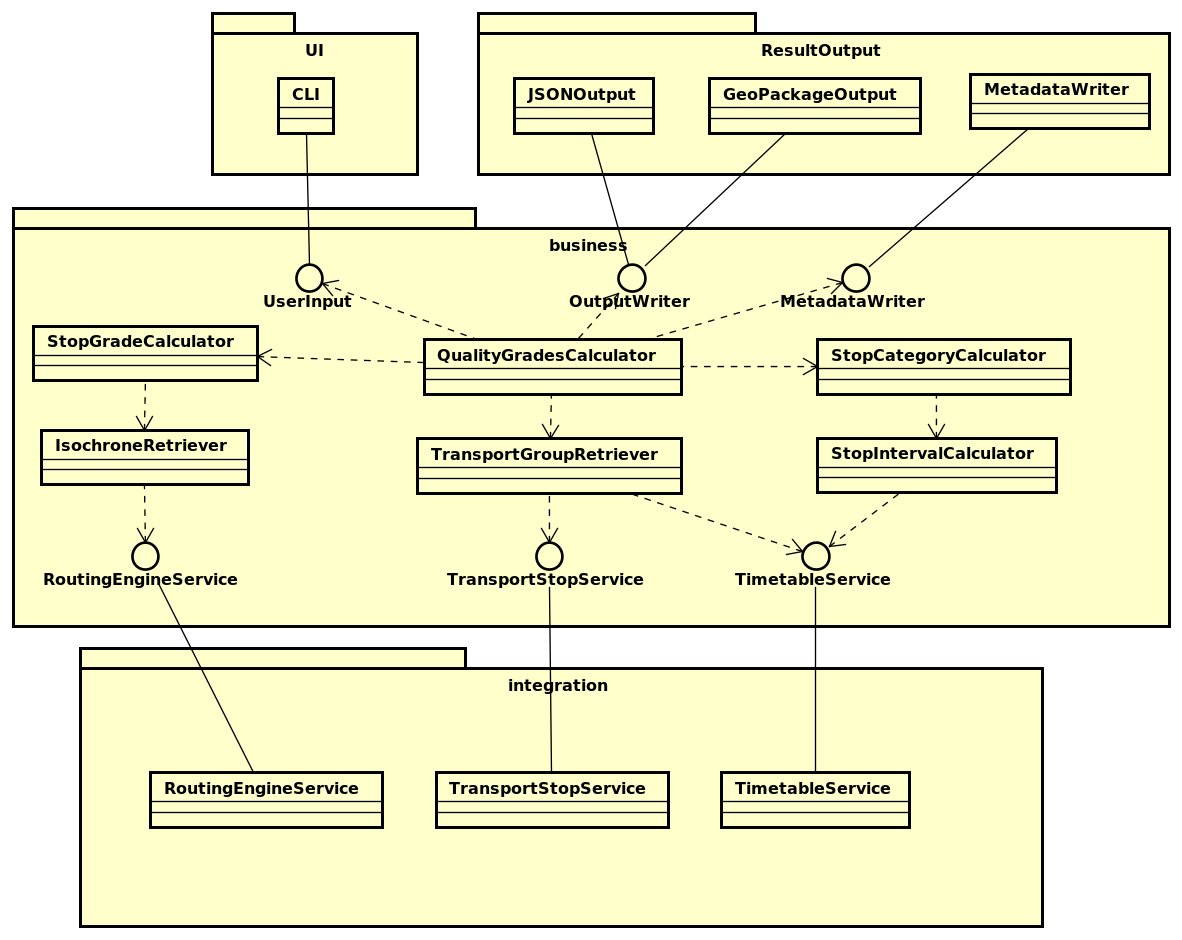
\includegraphics[width=1.0\linewidth]{projectdoc/img/guetklassen_generator_architektur.png}
    \caption[Schichten-Diagramm ÖV-Güteklassen Generator]{Schichten-Diagramm ÖV-Güteklassen Generator}
    \label{fig:layer_diagram_generator}
\end{figure}

Die Softwarearchitektur ist an die "`Clean Architecture"'-Prinzipien von \cite{martin_clean_architecture} angelehnt.
Diese Architektur hat den Vorteil, dass die Kernlogik, die business-Schicht, keine Abhängigkeiten auf die die anderen Schichten hat.
Diese Schicht ist somit absolut unabhängig.
Durch das Exponieren von Interfaces für die Schichten darüber und darunter können diese separat mit unterschiedlichen Dynamiken entwickelt werden.
So entsteht beispielsweise der Anspruch nach einem zusätzlichen Output-Format öfters als nach einer Anpassung der Berechnung der \acs{ÖV}-Güteklassen.
Durch diese Trennung kann nun die Schicht \nameref{layer:output} um einen zusätzlichen Service ergänzt werden ohne Gefahr zu laufen, dass die Kernlogik durch die Änderung unbemerkt vom bisherigen Verhalten abweicht.
Die Kernlogik erwartet grundsätzlich nur eine Implementation, welche das bereitgestellte Interface implementiert.
Wie sie dieses Interface implementiert ist der business-Schicht prinzipiell egal.
Im Folgenden werden die einzelnen Schichten beschrieben.

\paragraph{business}~\\
\label{layer:business}
In dieser Schicht ist die Kernlogik des Generators angesiedelt.
Hier wird die Berechnung der \acs{ÖV}-Güteklassen koordiniert.
So wird die Konfiguration des Users entgegen genommen und die nötigen Vorverarbeitungen und Berechnungen angestossen.
Durch die Natur der Berechnungslogik (siehe Abbildung \ref{fig:Flow_OeVGK_Brechnung}) lässt sich die Logik analog strukturieren.
Dabei wird die Haltestellekategorie, welche sich aus der Art des VerkehrsmittelS und dem Kursintervall zusammensetzt, über den Service \emph{StopCategoryCalculator} berechnet.
Die \acs{ÖV}-Güteklassen lassen sich in einem weiteren Schritt mithilfe des \emph{StopGradeCalculator} berechnen.
\emph{QualityGradesCalculator} übernimmt hier die Koordination der Berechnung.

\paragraph{integration}~\\
\label{layer:integration}
Alle Datenbankzugriffe erfolgen über die Integration-Schicht.
Es ist bewusst kein \acl{ORM} angedacht.
Dies aus dem Grund, da intensiv mit StoredProcedures gearbeitet wird und vorallem Berechnungen auf der Datenbank durchgeführt werden und somit die Tabellen keine Objekte repräsentieren.

\paragraph{ui}~\\
\label{layer:ui}
In der ui-Schicht sind die Interaktionen mit dem User angedacht.
So ist hier ein CLI angesiedelt, welche Konfigurationen über eine einfache Bedienung entgegen nimmt.

\paragraph{output}~\\
\label{layer:output}
Die Ergebnisse der \acs{ÖV}-Güteklassen werden über diese Schicht dem User exponiert.
Der Vorteil der oben beschriebenen "`Plugin-Architektur"' macht sich hier stark sichtbar.
Entsteht das Verlangen nach einem zusätzlichen Output der \acs{ÖV}-Güteklassen, etwa als GeoPackage, kann problemlos ein Service \emph{GeoPackageWriter} erstellt werden, welche das Interface \emph{OutputWriter} implementiert und analog zum \emph{GeoJSONWriter} das Resultat als GeoPackage ausliefert.
Die Kernlogik in der business-Schicht muss so nicht angepasst werden.

Der \emph{MetadataWriter} ist gesondert hervorzuheben.
Durch diesen werden Konsumenten des Resultats des "`\acs{ÖV}-Güteklassen 2018 Generator"' darüber informiert, welche \acs{ÖV}-Güteklassen generiert wurden, sprich für welche Stichtage und Zeitintervalle liegt ein Ergebnis vor.
Dabei handelt es sich um eine JSON-Datei.

\subsubsection{Backend}
\label{container:Backend}

Das Backend nimmt die Ergebnisse der Berechnungen vom Container \nameref{container:generator} entgegen.
Konkret heisst das, dass das Backend die Metadaten, welche vom Container \nameref{container:generator} zusätzlich zu den \acs{ÖV}-Güteklassen geschrieben werden, einliest und diese Daten über eine Web-\ac{API} möglichen Clients zur Verfügung stellt.
Das Web-\ac{API} exponiert somit die Information über welche Stichtage und Zeitintervalle \acs{ÖV}-Güteklassen vorhanden sind.

Über das Backend werden nicht direkt die generierten \acs{ÖV}-Güteklassen beispielsweise als GeoJSON ausgeliefert.
Dies aus dem Grund, da diese Dateien eine Grösse haben, welche eine Auslieferung über ein Web-\ac{API} nicht zumutbar machen.
Für die Visualisierung auf einer Karte eignen sich andere Varianten, welche in den Container \nameref{container:Web-App} und \nameref{container:Tile-Server} angesprochen werden.

\paragraph{Web-\ac{API}}
Die Services, welche über das Web-\ac{API} exponiert werden, sind in Tabelle \ref{table:Wep-API} aufgeführt.

\begin{table}[H]
    \centering
    \begin{tabular}[c]{l l p{10.5cm}}
        \toprule
        \textbf{Route}          
                                & \textbf{Argument}
                                & \textbf{Zweck}\\
        \midrule
        \emph{/typesOfDays}
                                & -
                                & Retourniert die Stichtage für welche \acs{ÖV}-Güteklassen vorhanden sind.\\
        \emph{/gradings}        & typeOfDay
                                & Retourniert die Zeitintervalle, welche für den übergebenen Stichtag (typeOfDay) vorhanden sind.\\
        \bottomrule
    \end{tabular}
    \caption{Web-\ac{API}}
    \label{table:Wep-API}
\end{table}


\subsubsection{Web-App}
\label{container:Web-App}

Die Web-App dient als Frontend des Systems "`\acs{ÖV}-Güteklassen 2018"'.
Die Applikation wird als \ac{SPA} direkt an den Browser des Users ausgeliefert.
Die Web-App nutzt das \ac{API} des \nameref{container:Backend}-Containers für das Beziehen von Metadaten, welche die verfügbaren ÖV-Güteklassen beschreiben.
Mithilfe der Metadaten können die ÖV-Güteklassen vom Container \nameref{container:Tile-Server} bezogen und visualisiert werden.

Dafür wird, wie in den Rahmenbedingungen (Kap. \ref{Einführung:Rahmenbedingungen, Umfeld, Definitionen, Abgrenzungen}) festgehalten, entweder \emph{Vue.js}~\cite{vuejs} oder \emph{React}~\cite{react} verwendet.
Die beiden Varianten wurden im Kapitel \ref{Analyse:Evaluation Frontend-Framework} evaluiert.

\subsubsection{Tile-Server}
\label{container:Tile-Server}

Die berechneten \acs{ÖV}-Güteklassen werden als Vector Tiles~\cite{geometalab_vectortiles} ausgeliefert.
Der Grund dafür ist, dass die Performanz um einiges besser ist, als wenn man direkt ein GeoJSON oder Raster-Kacheln ausliefert, da unteranderm nur der gerade geforderte Auszug geladen wird und bei unterschiedlichen Zoom-Stufen skaliert werden kann.
Davon verspricht man sich ein bessere Usability, da die \acs{ÖV}-Güteklassen je nach Position und Zoom-Stufe schneller verfügbar sind.
Ebenfalls muss das Frontend keine grosse Dateien vom Backend laden, was bei der Visualisierung eines GeoJSON der Fall wäre.

Damit der Container \nameref{container:Web-App} Vector-Tiles von den generierten \acs{ÖV}-Güteklassen beziehen kann, müssen diese über einen Tile-Server exponiert werden.

\subsubsection{Routing-Engine}
\label{container:Routing-Engine}

Die Routing-Engine ist für die Berechnung von Isolinien verantwortlich.
Dazu werden zuerst periodisch die Kartendaten von \nameref{subsystem:planet.osm.ch} eingelesen und zusammen mit dem \gls{Terrainmodell} von \nameref{subsystem:swissALTI3D}, das zuvor vom Admin manuell besorgt wurde, eine Routing-Topologie erstellt.

Sobald der Admin die Berechnung der ÖV-Güteklassen auslöst, wird die Routing-Engine vom \nameref{container:generator} nach Isolinien abgefragt, die mit Haltestellen als Startpunkt und einer gewissen Distanz (gewichtet nach Höhenunterschied) berechnet werden.
Diese Isodistanzen bilden Polygone, die anschliessend vom Generator weiter verarbeitet werden.


\subsection{Code}
\label{Architektur:Code}

%TODO vlt. auf anderes Kapitel verweisen